\documentclass{beamer}
\usepackage{tabularx}
\usepackage{graphicx}
%Information to be included in the title page:
\title{Design specification \newline Closed Aquaculture System}
%\author{Anonymous}
\institute{Operational systems - ScaleAQ}
\date{\today}

\begin{document}

\frame{\titlepage}

\begin{frame}
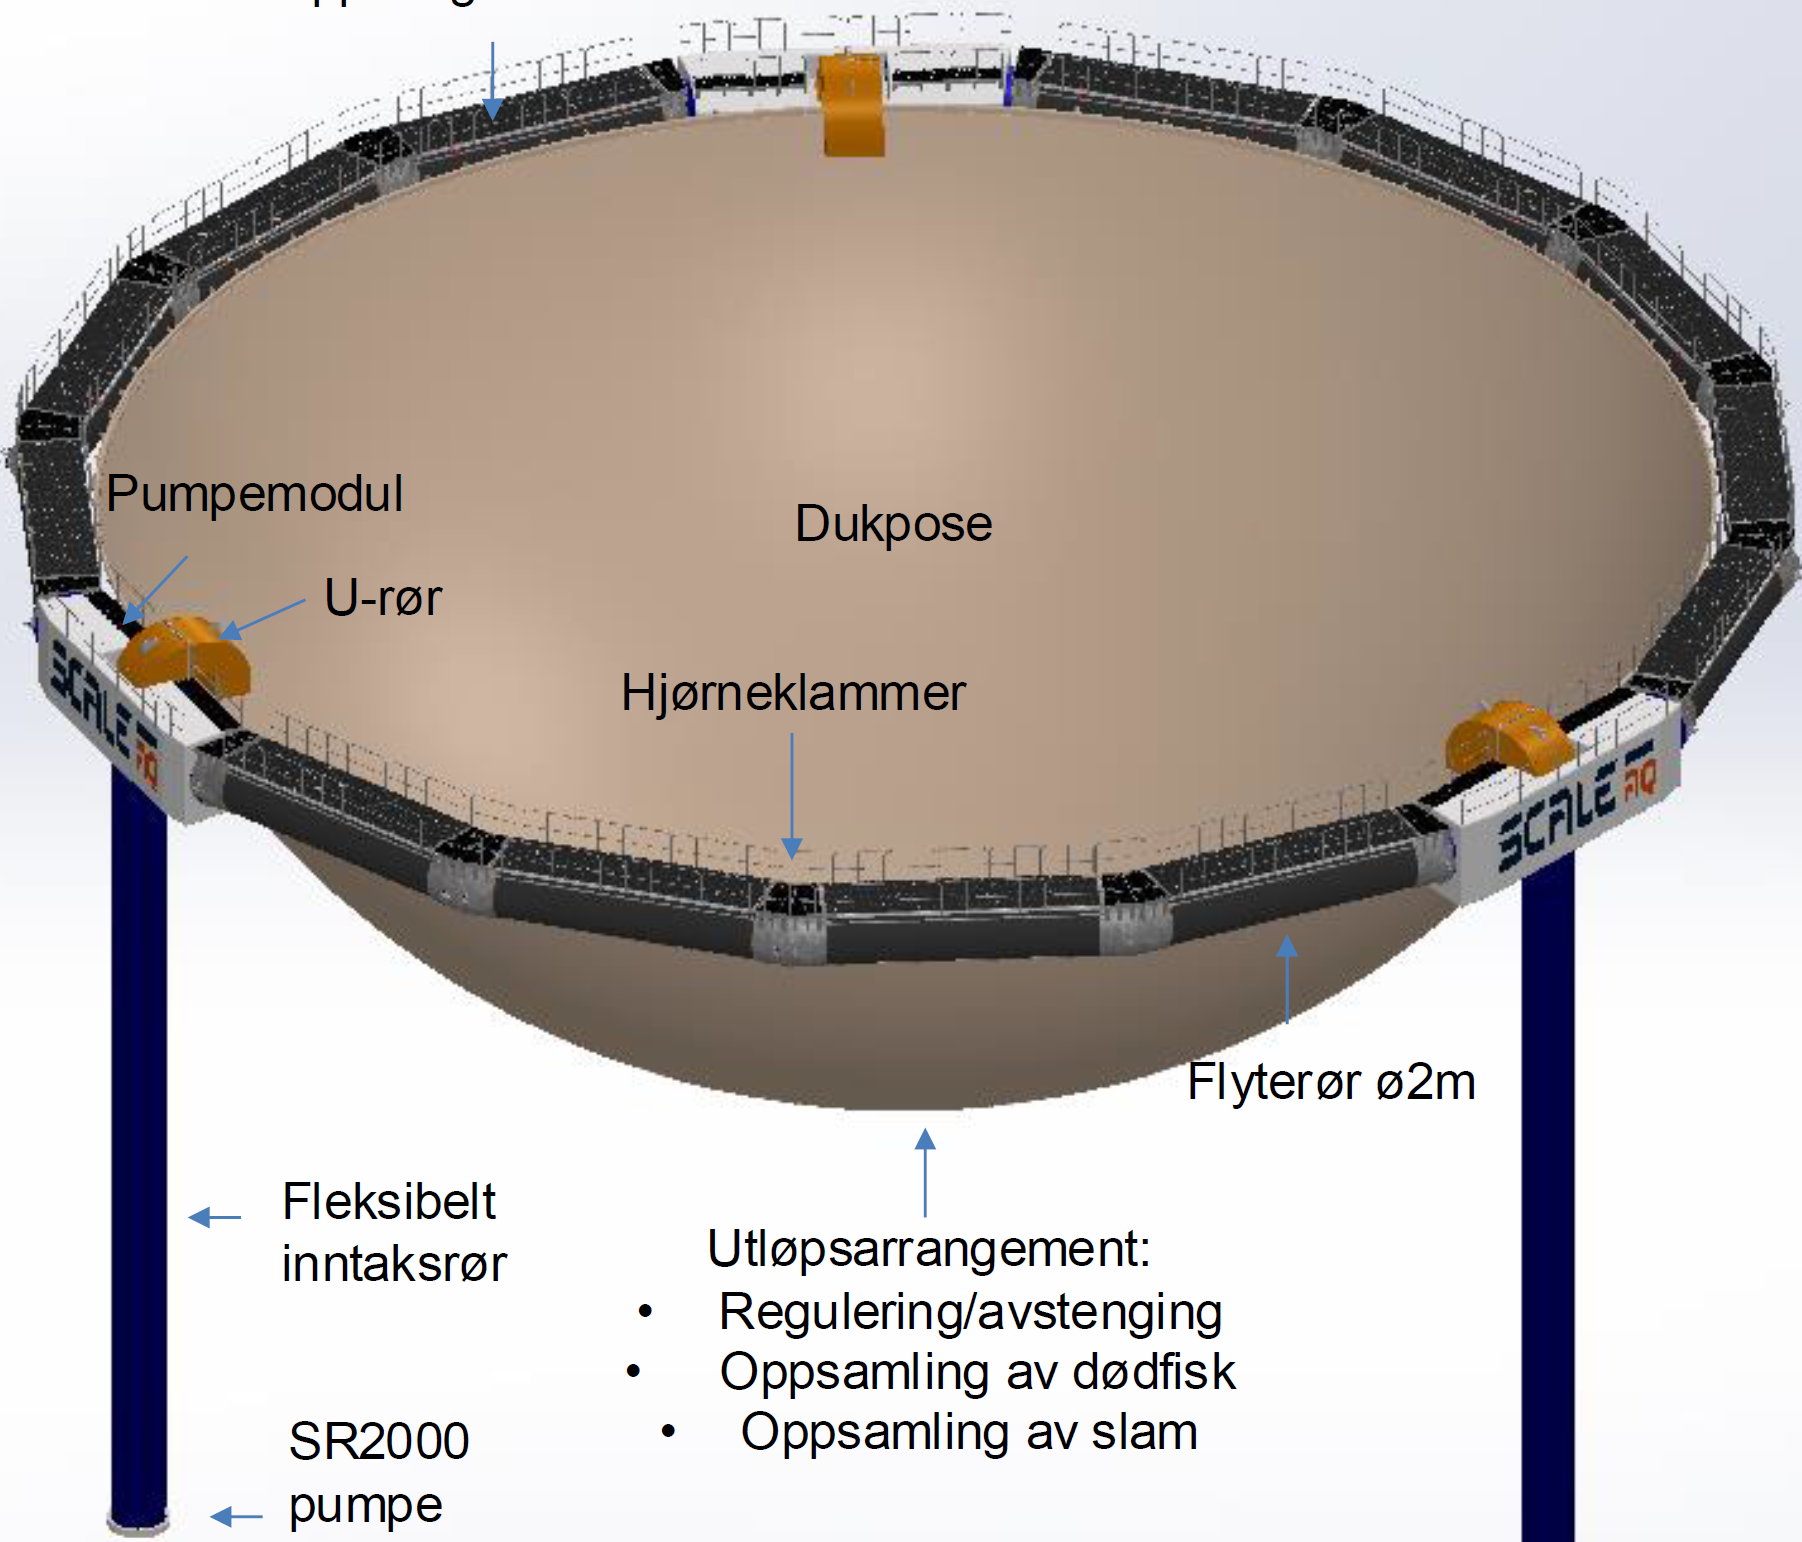
\includegraphics [width=.9\textwidth]{cas.png}
\end{frame}

\begin{frame}
\frametitle{Functional requirements}
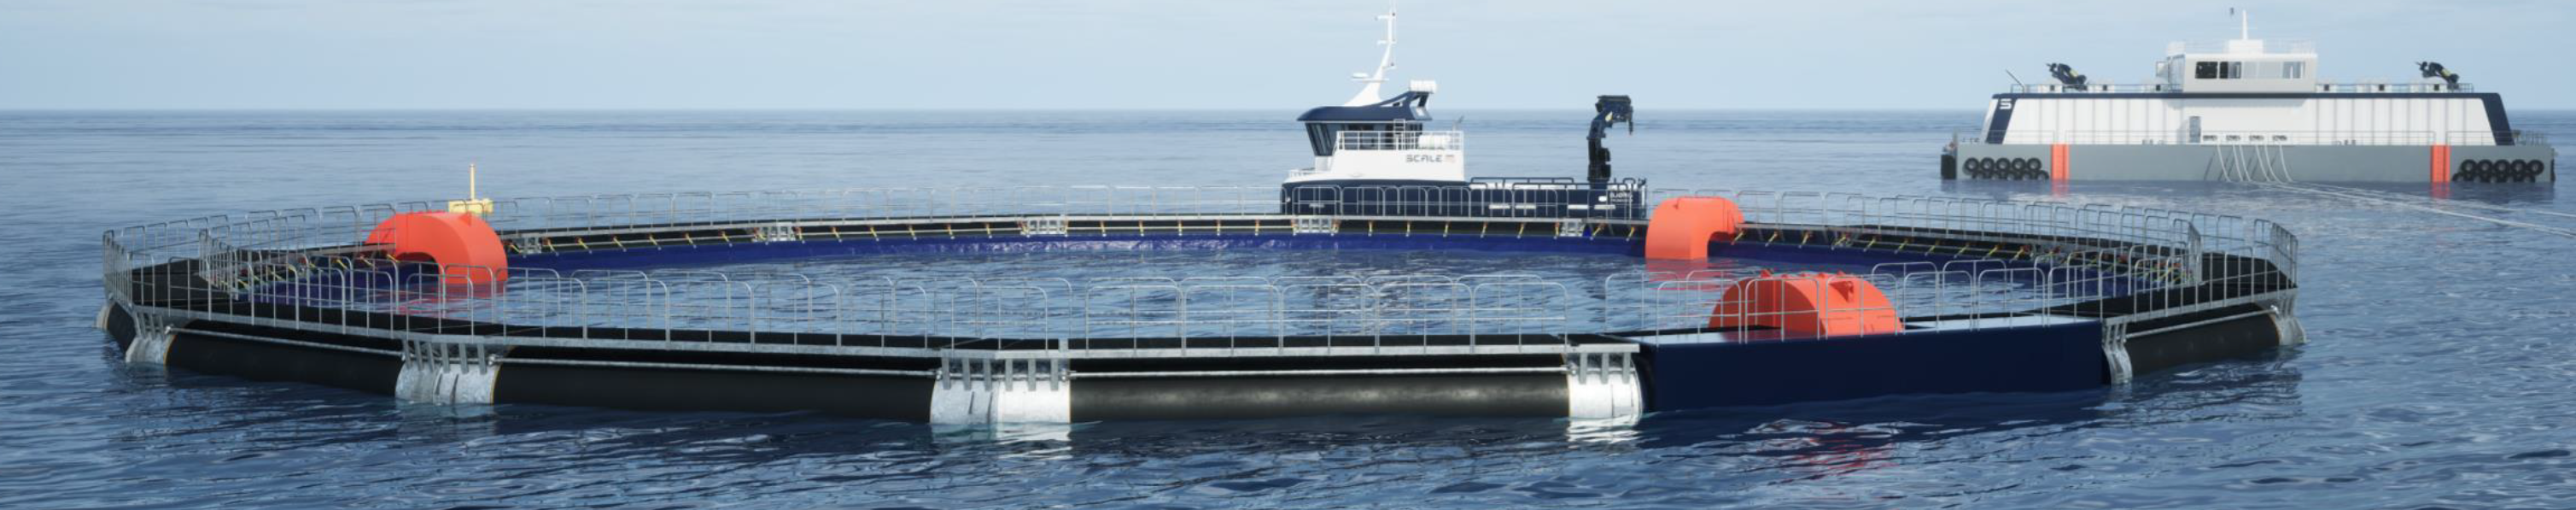
\includegraphics [width=\textwidth]{cas_top.png}
\tiny \textbf{FUNCTIONAL REQUIREMENT SPECIFICATION FOR PUMP\\ INLET SYSTEM: Level control}\\[.2cm]
\tiny
\begin{tabularx}{\textwidth}{llX}
1. &Process: &Regulate the internal water level relative to the outer sea level (delta height). Required to accurate measure levels down to 1mm.\\[.2cm]
2. & Inputs: &\textit{Field instruments}: \newline Pressure, distance (ultrasonic), RPM, Power, valve position \newline \textit{User}: \newline delta height set point, RPM, regulator parameters, control commands\\[.5cm]
3. &Outputs: & RPM control signal to pumps, control commands to FRAMO PLC controller\\[.2cm]
4. &Major error: & Loss of IO inputs, fatal error on VSD's, disturbance due to weather/waves\\[.2cm]
5. &Exception response & Switch to manual operation with default values, trip VSD (2oo3) 
\end{tabularx}
\end{frame}

\begin{frame}

\frametitle{Functional requirements}
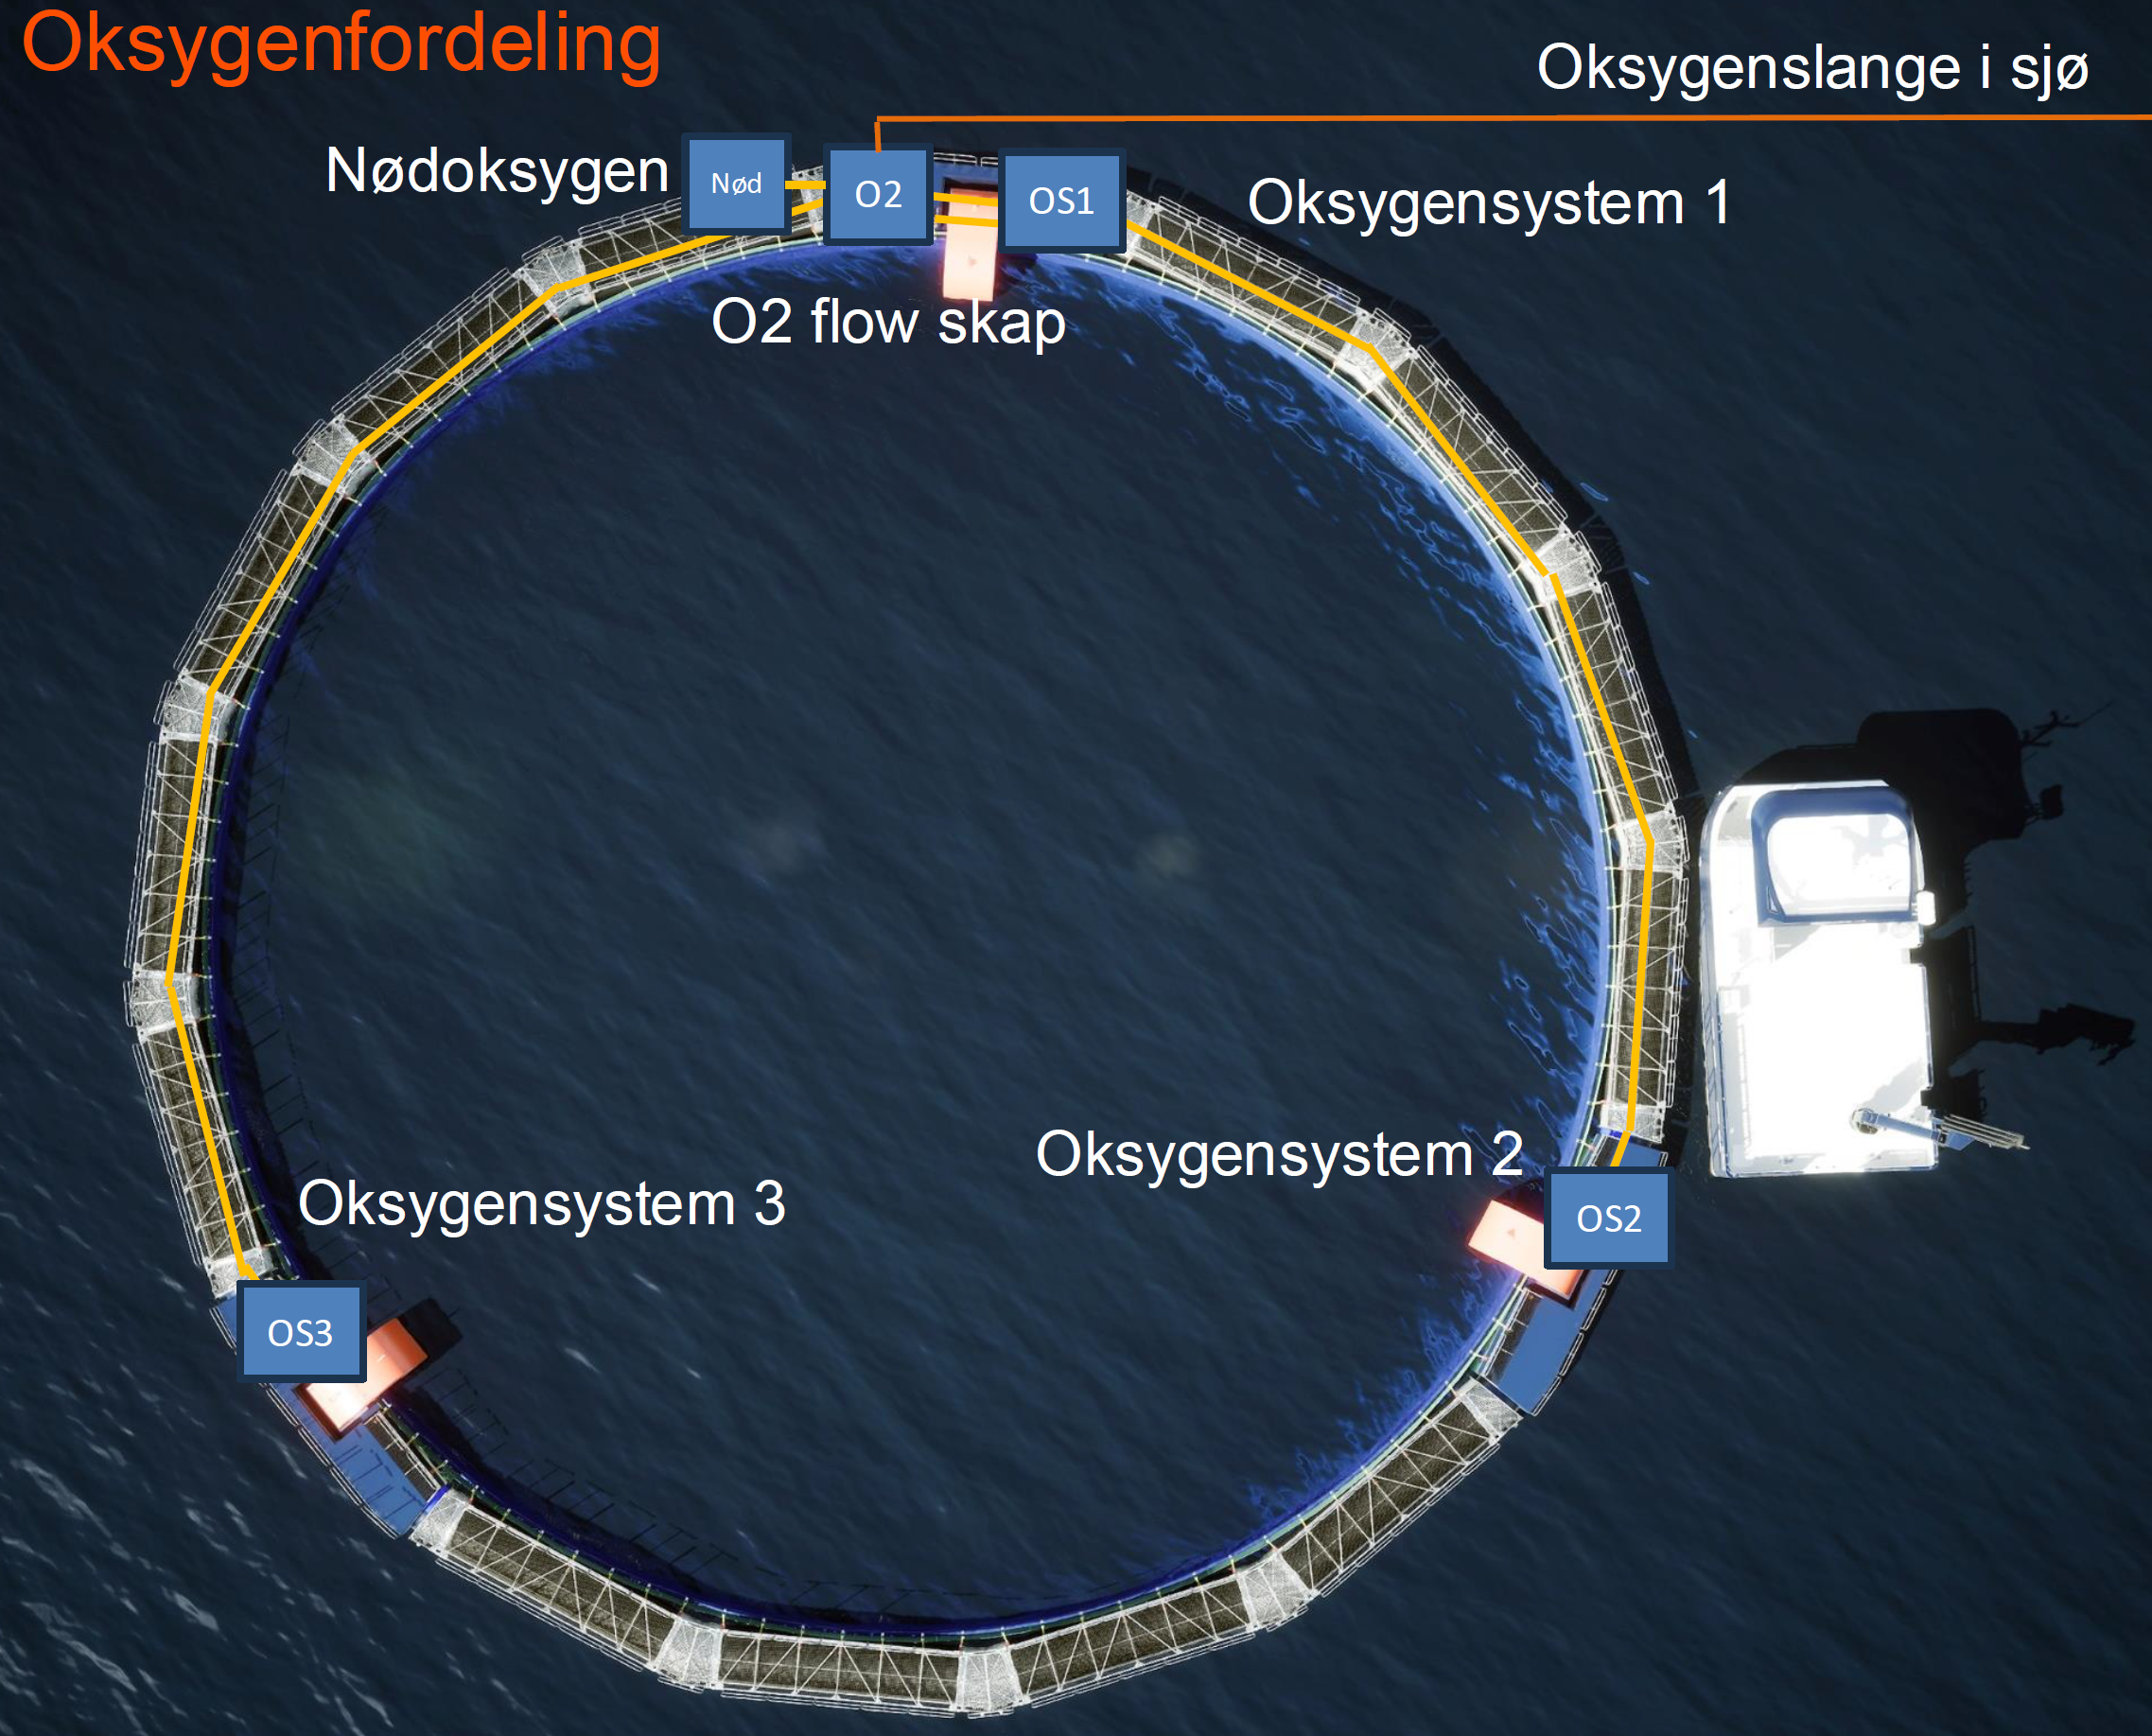
\includegraphics [width=.5\textwidth]{cas_top_oxy.png} \newline
\tiny \textbf{FUNCTIONAL REQUIREMENT SPECIFICATION FOR OXYGENATOR INJECTOR}\\[.2cm]
\tiny
\begin{tabularx}{\textwidth}{llX}
1. &Process: &Inject oxygen into branch of each inlet pump.\\[.2cm]
2. &Inputs: &\textit{Field instruments}: \newline $O_2$ concentration, pressure, \newline \textit{User}: \newline oxygen concentration set point, regulator parameters, oxygen control valve position\\[.2cm]
3. &Outputs: & RPM control signal to pumps, control commands to FRAMO PLC controller\\[.2cm]
4. &Major error: & Loss of oxygen reading, loss of pump speed, control valve / solenoid malfunction, centrifugal pump/VSD error\\[.2cm]
5. &Exception response & Switch to manual operation with default values, trip oxygenator system
\end{tabularx}
\end{frame}

\begin{frame}
\frametitle{Functional requirements}
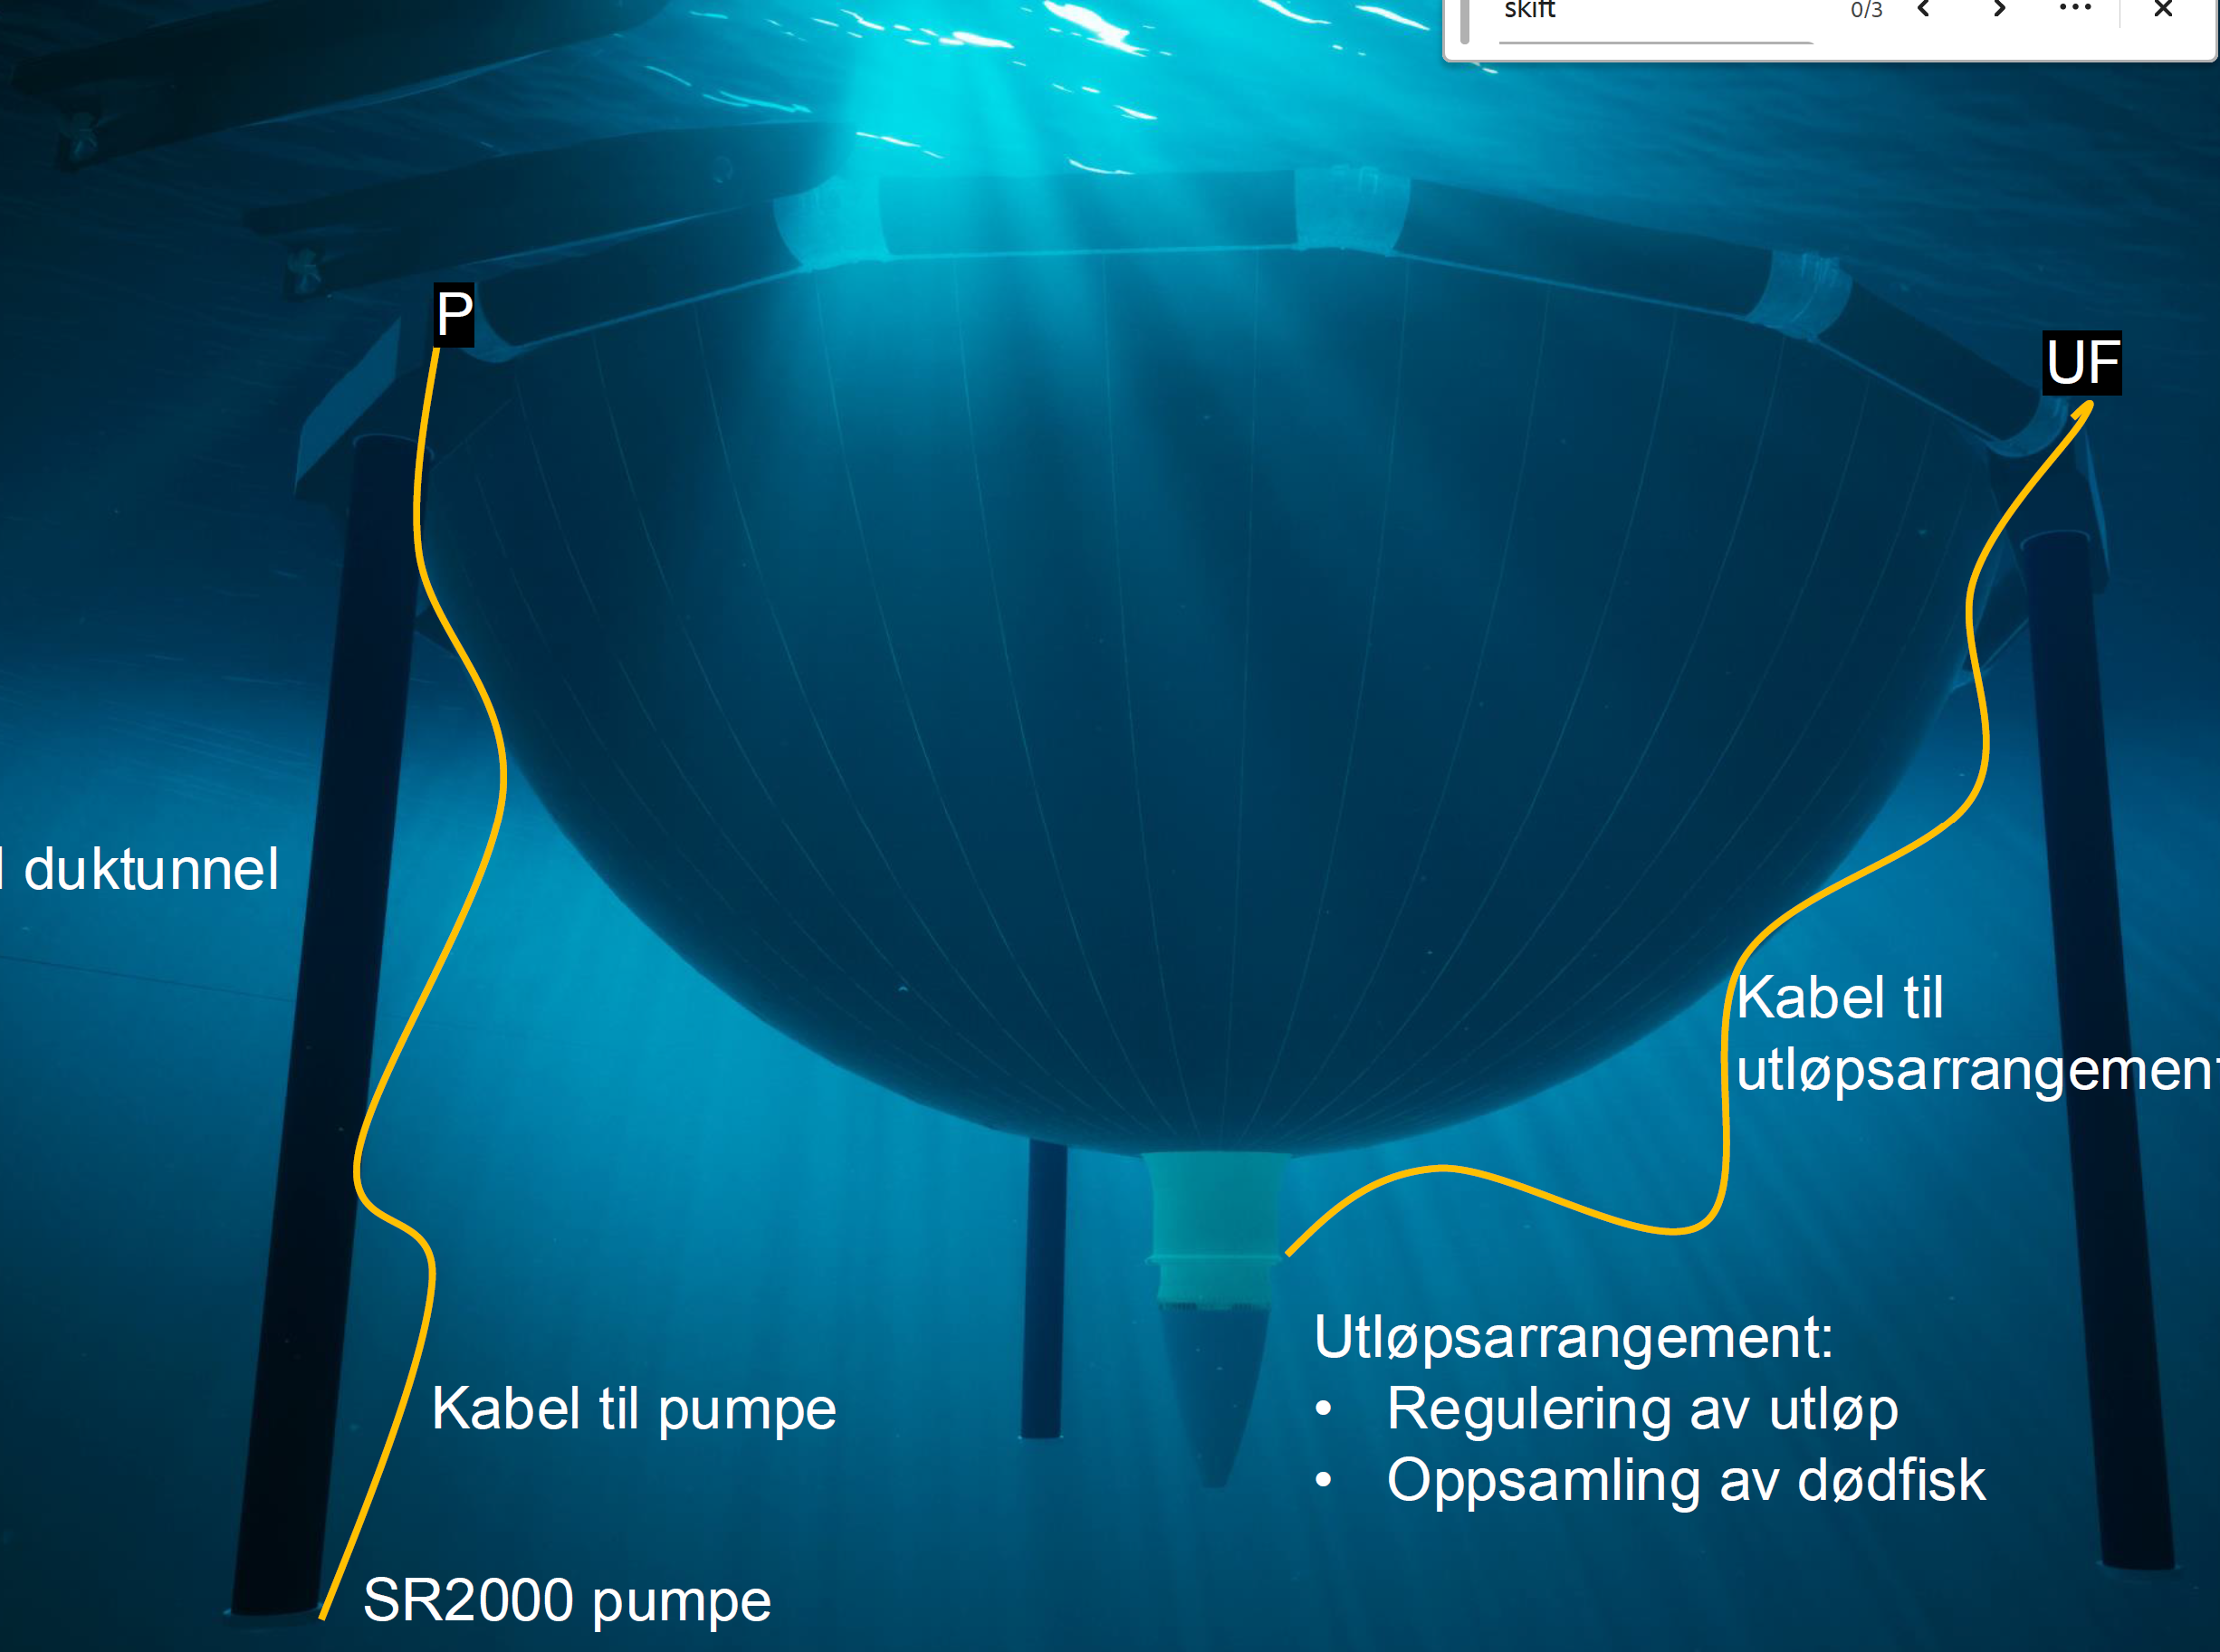
\includegraphics [width=.5\textwidth]{cas_subsea.png} \newline
\tiny \textbf{FUNCTIONAL REQUIREMENT SPECIFICATION FOR OUTLET VALVE}\\[.2cm]
\tiny
\begin{tabularx}{\textwidth}{llX}
1. &Process: & Control the water exchange rate \\[.2cm]
2. & Inputs: &\textit{Field instruments}: \newline Outlet valve position, RPM of inlet pumps, power consumptin inlet pumps \newline \textit{User}: \newline  set point position outlet valve \\[.2cm]
3. &Outputs: & Control signal to outlet valve\\[.2cm]
4. &Major error: &Loss of inlet pumps, outlet valve malfunction, clogging\\[.2cm]
5. &Exception response & Close outlet valve, trip inlet pumps, reduce water level height on inlet pump system\\[.2cm]
\end{tabularx}
\end{frame}

\begin{frame}
\frametitle{Scenarios}
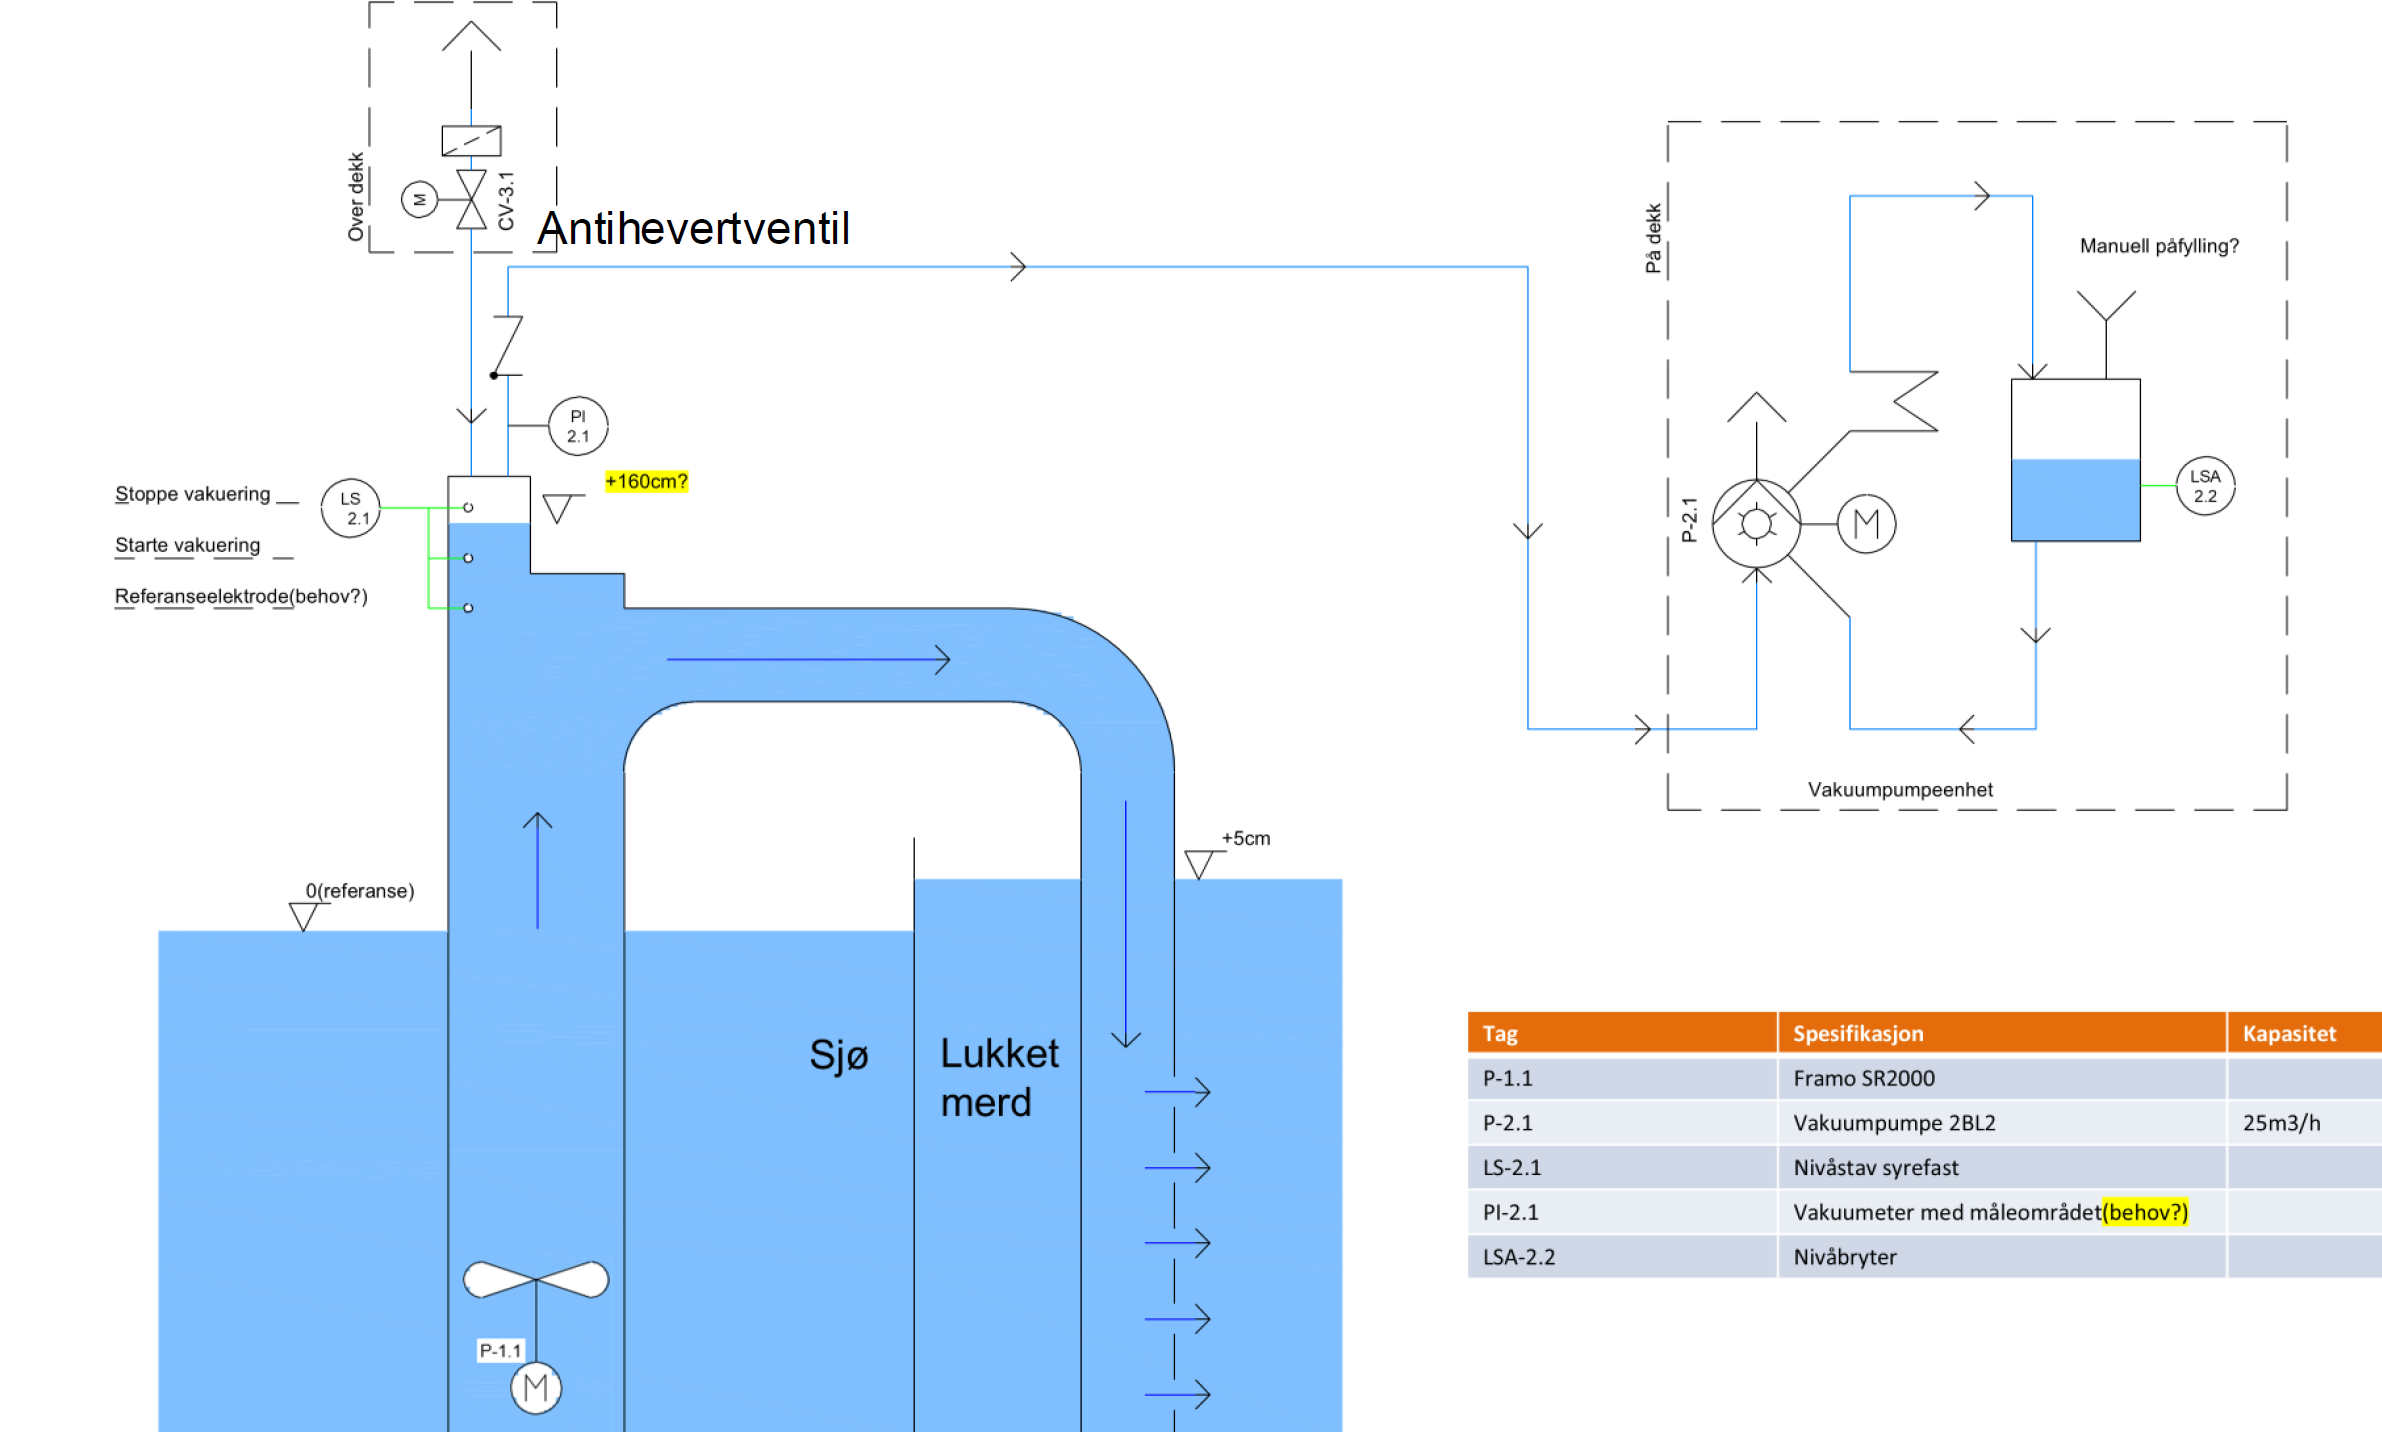
\includegraphics [width=.53\textwidth]{siphon.png} \newline
\framebox{\parbox{\dimexpr\linewidth-2\fboxsep-2\fboxrule}{
\scriptsize \begin{enumerate}
\item<1-> All systems are powered up and outlet valve is in position within valid range.
\item<2-> User sends start command to pump no. 1
\item<3-> System checks condition of process and begins the starting sequence of inlet pump.
\item<4-> The pumps starts at reduced speed, vacuum system starts and anti-siphon valve closes.
\item<5-> After a limit switch at outlet piping triggers, the vacuum pump stops and the pump starts running at reduced speed
\item<6-> System changes to "remote operation" and in "manual mode" at 50 RPM.
\end{enumerate}
\textbf{Finish}
\vspace{0.1cm}
\hrule
\vspace{0.1cm}
Scenario 1 - Cold start of inlet pump no. 1 into manual operation mode at a given speed.
  }}


\end{frame}

\begin{frame}
\frametitle{Scenarios}
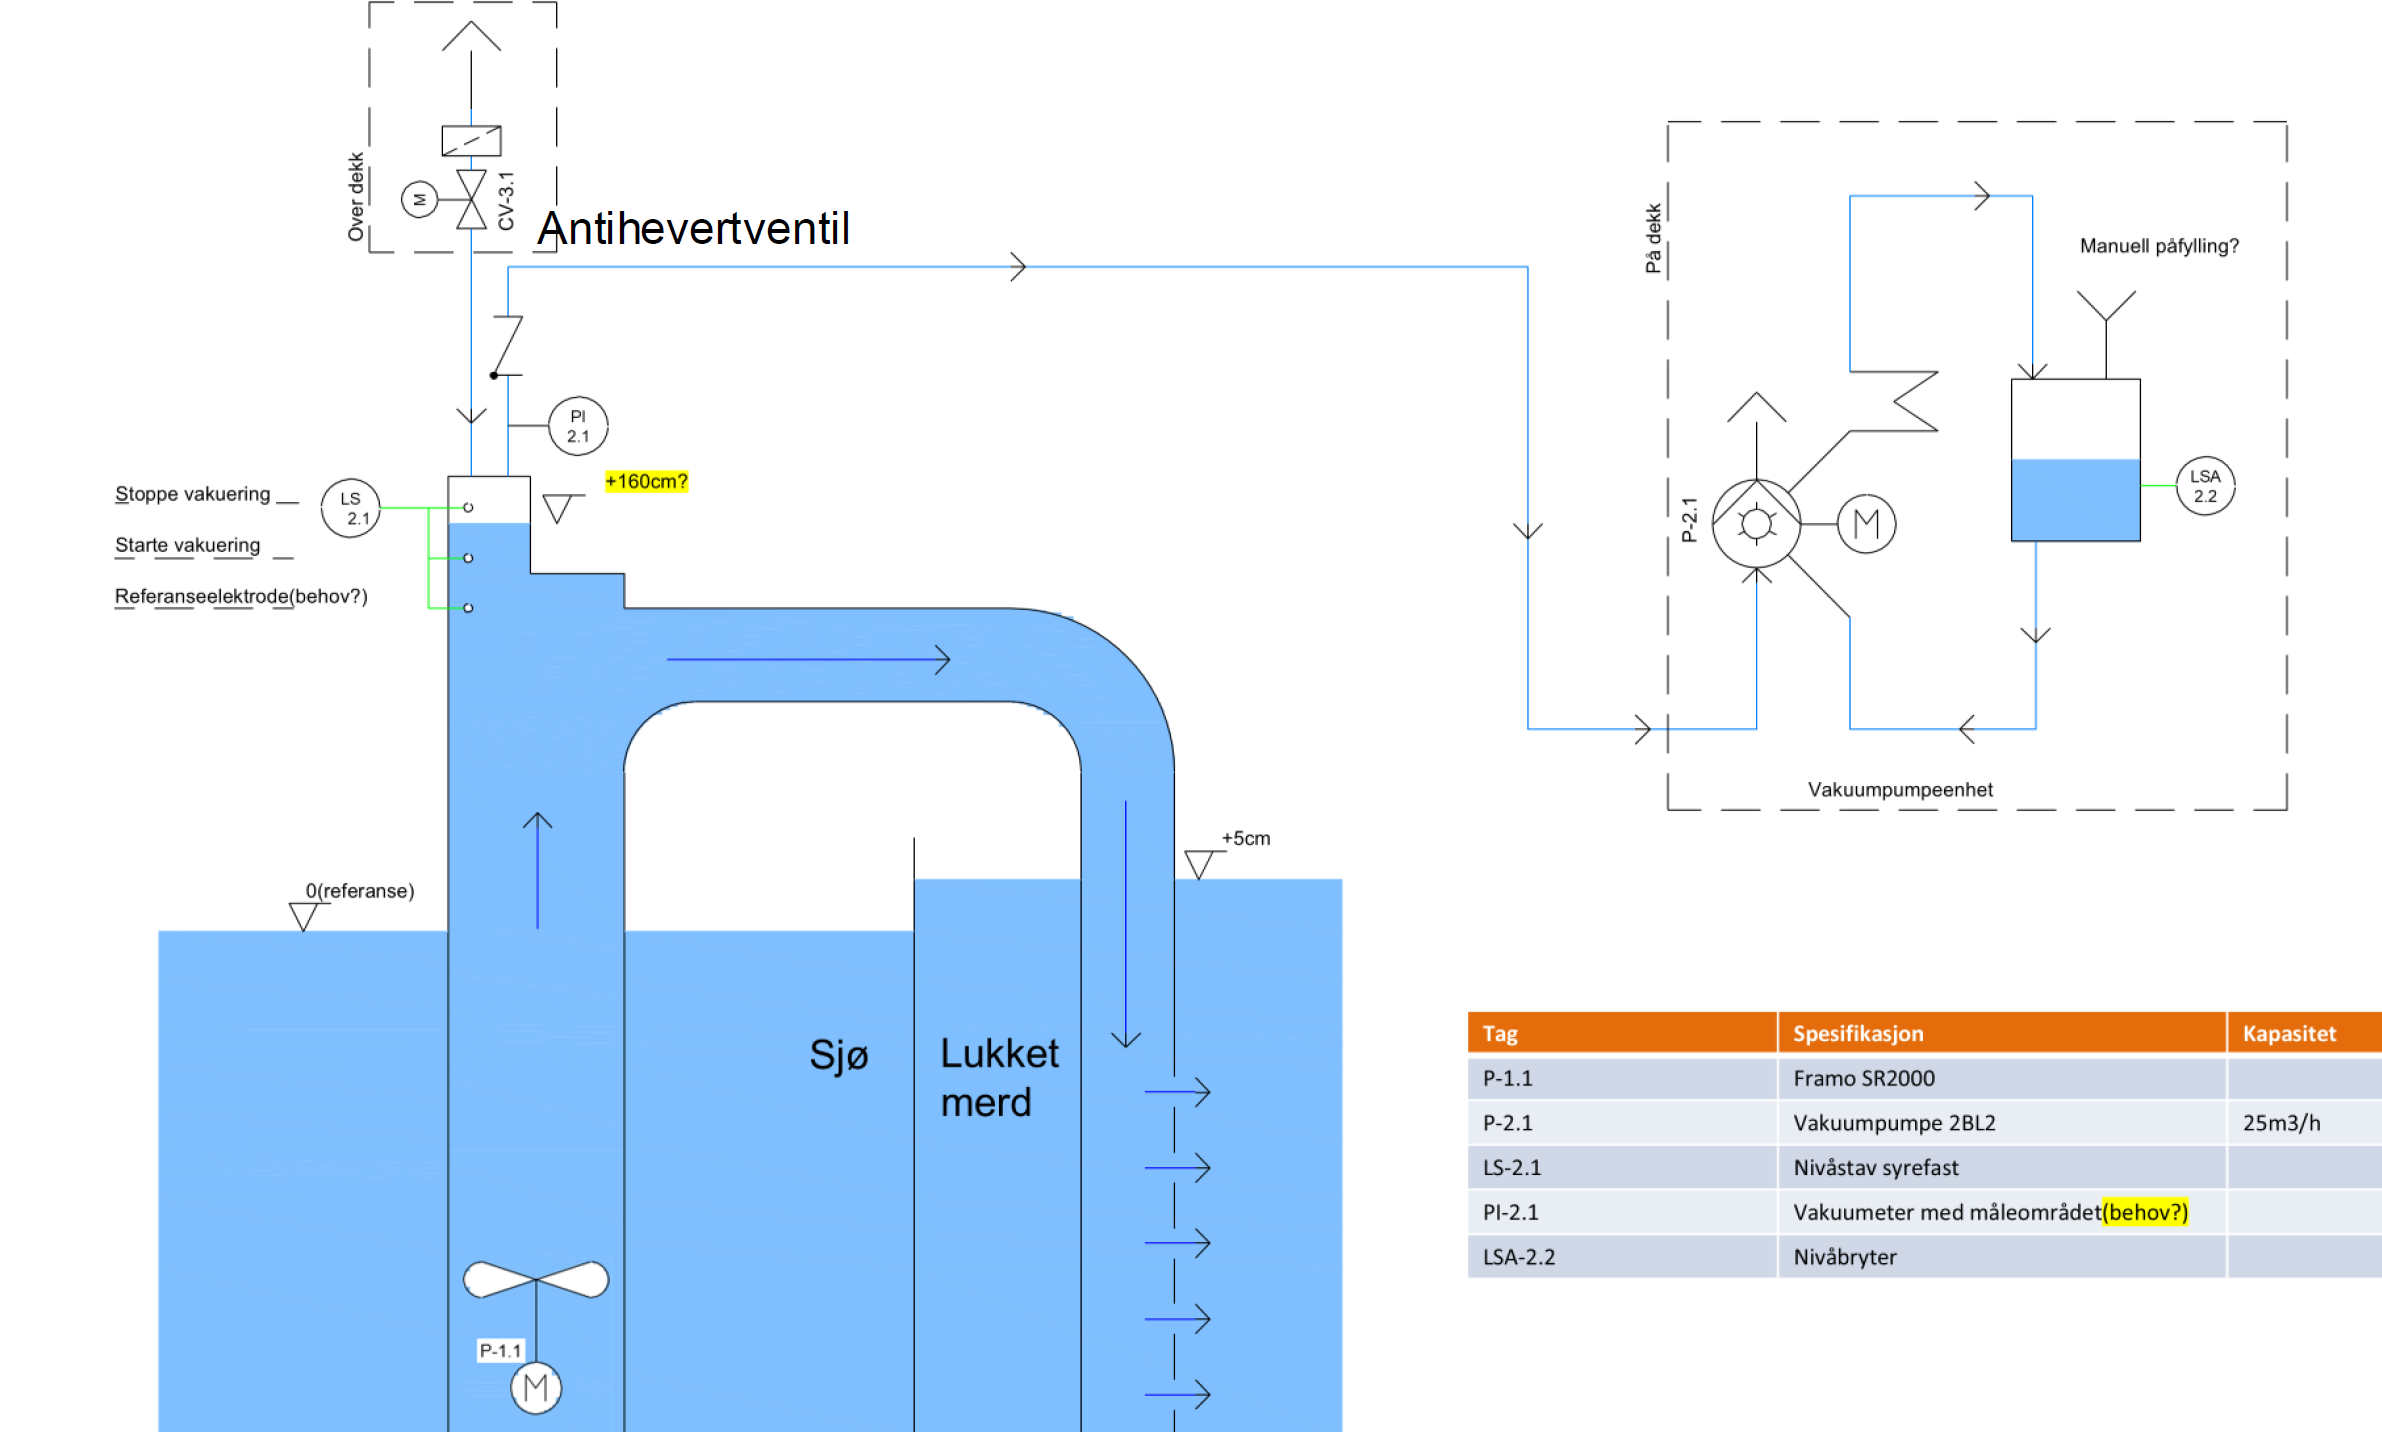
\includegraphics [width=.53\textwidth]{siphon.png} \newline
\framebox{\parbox{\dimexpr\linewidth-2\fboxsep-2\fboxrule}{
\scriptsize \begin{enumerate}
\item<1-> All systems are powered up and outlet valve is in position within valid range.
\item<2-> User sends start command to pump no. 1
\item<3-> System checks condition of process and begins the starting sequence of inlet pump.
\item<4-> The pumps starts at reduced speed, vacuum system starts and anti-siphon valve closes.
\item<5-> Limit switch has not triggered within the defined time.
\item<6-> System changes to "failed to start", stop command is sent to the pump and anti siphon valve opens.
\end{enumerate}
\textbf{Finish}
\vspace{0.1cm}
\hrule
\vspace{0.1cm}
Scenario 2 - Cold start of inlet pump no. 1 into failed to start state.
  }}

\end{frame}

\begin{frame}
\frametitle{Scenarios}
\onslide<4->{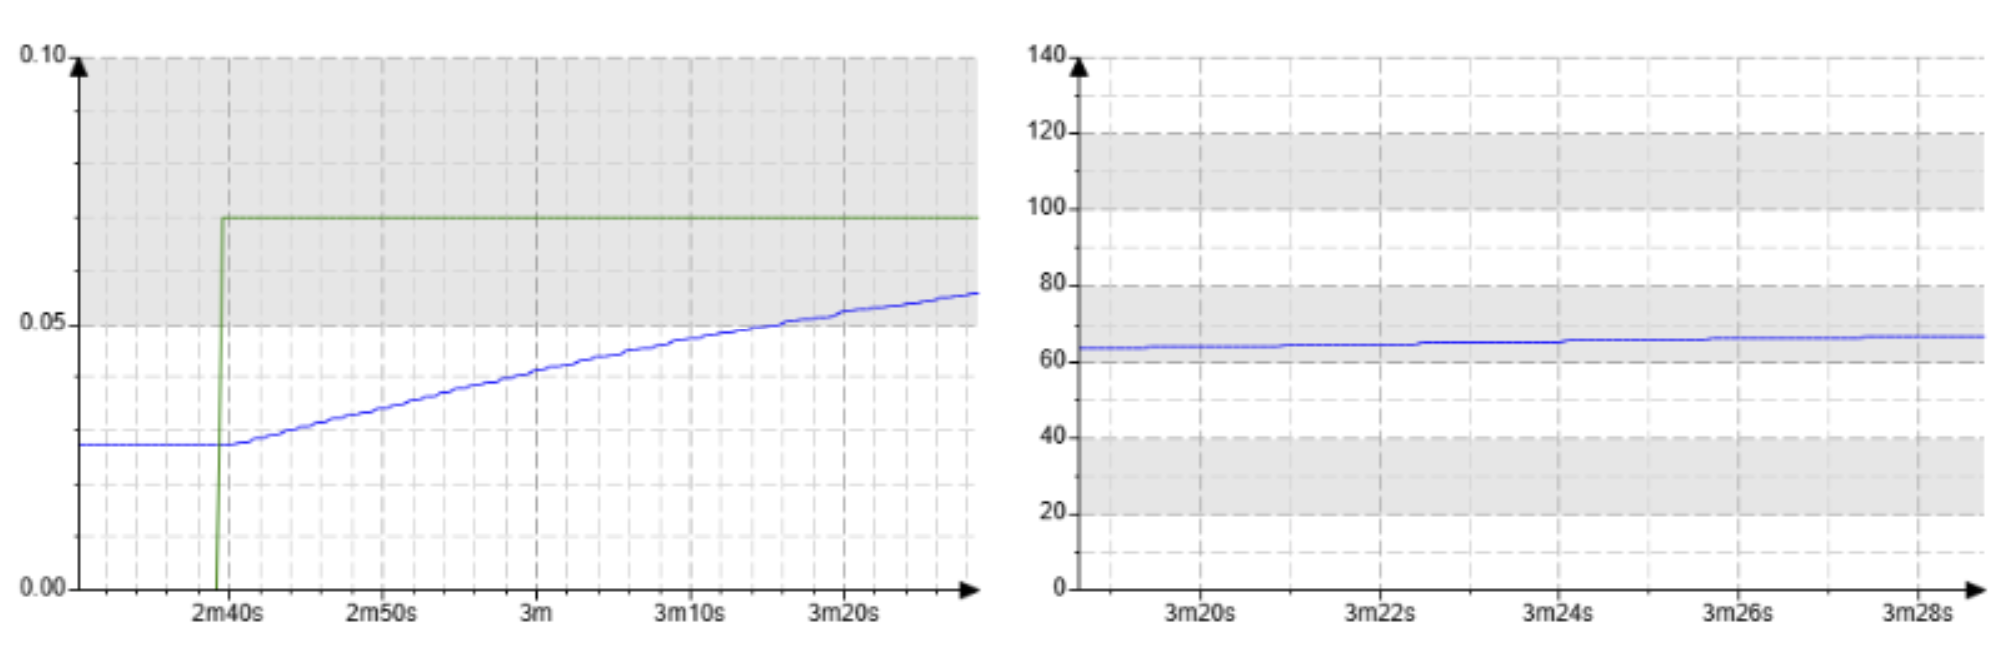
\includegraphics[width=\textwidth]{snip1.png}} \newline
\framebox{\parbox{\dimexpr\linewidth-2\fboxsep-2\fboxrule}{
\footnotesize \begin{enumerate}
\item<1-> All pumps have started and is running in remote operation at 50RPM.
\item<2-> Send auto command to controller.Verify that the controller set point is updated with the current value.
\item<3-> Verify that the RPM control signal to the pumps are stable at around 50RPM.
\item<4-> Change set point to 7cm. Verify that RPM control signal and delta height is stable and rising towards stationary values.
\end{enumerate}
\textbf{Finish}
\vspace{0.1cm}
\hrule
\vspace{0.1cm}
Scenario 3 - Putting the pumps in auto mode after startup and update the set point to the regulator.
  }}

\end{frame}

\begin{frame}
\frametitle{Scenarios}
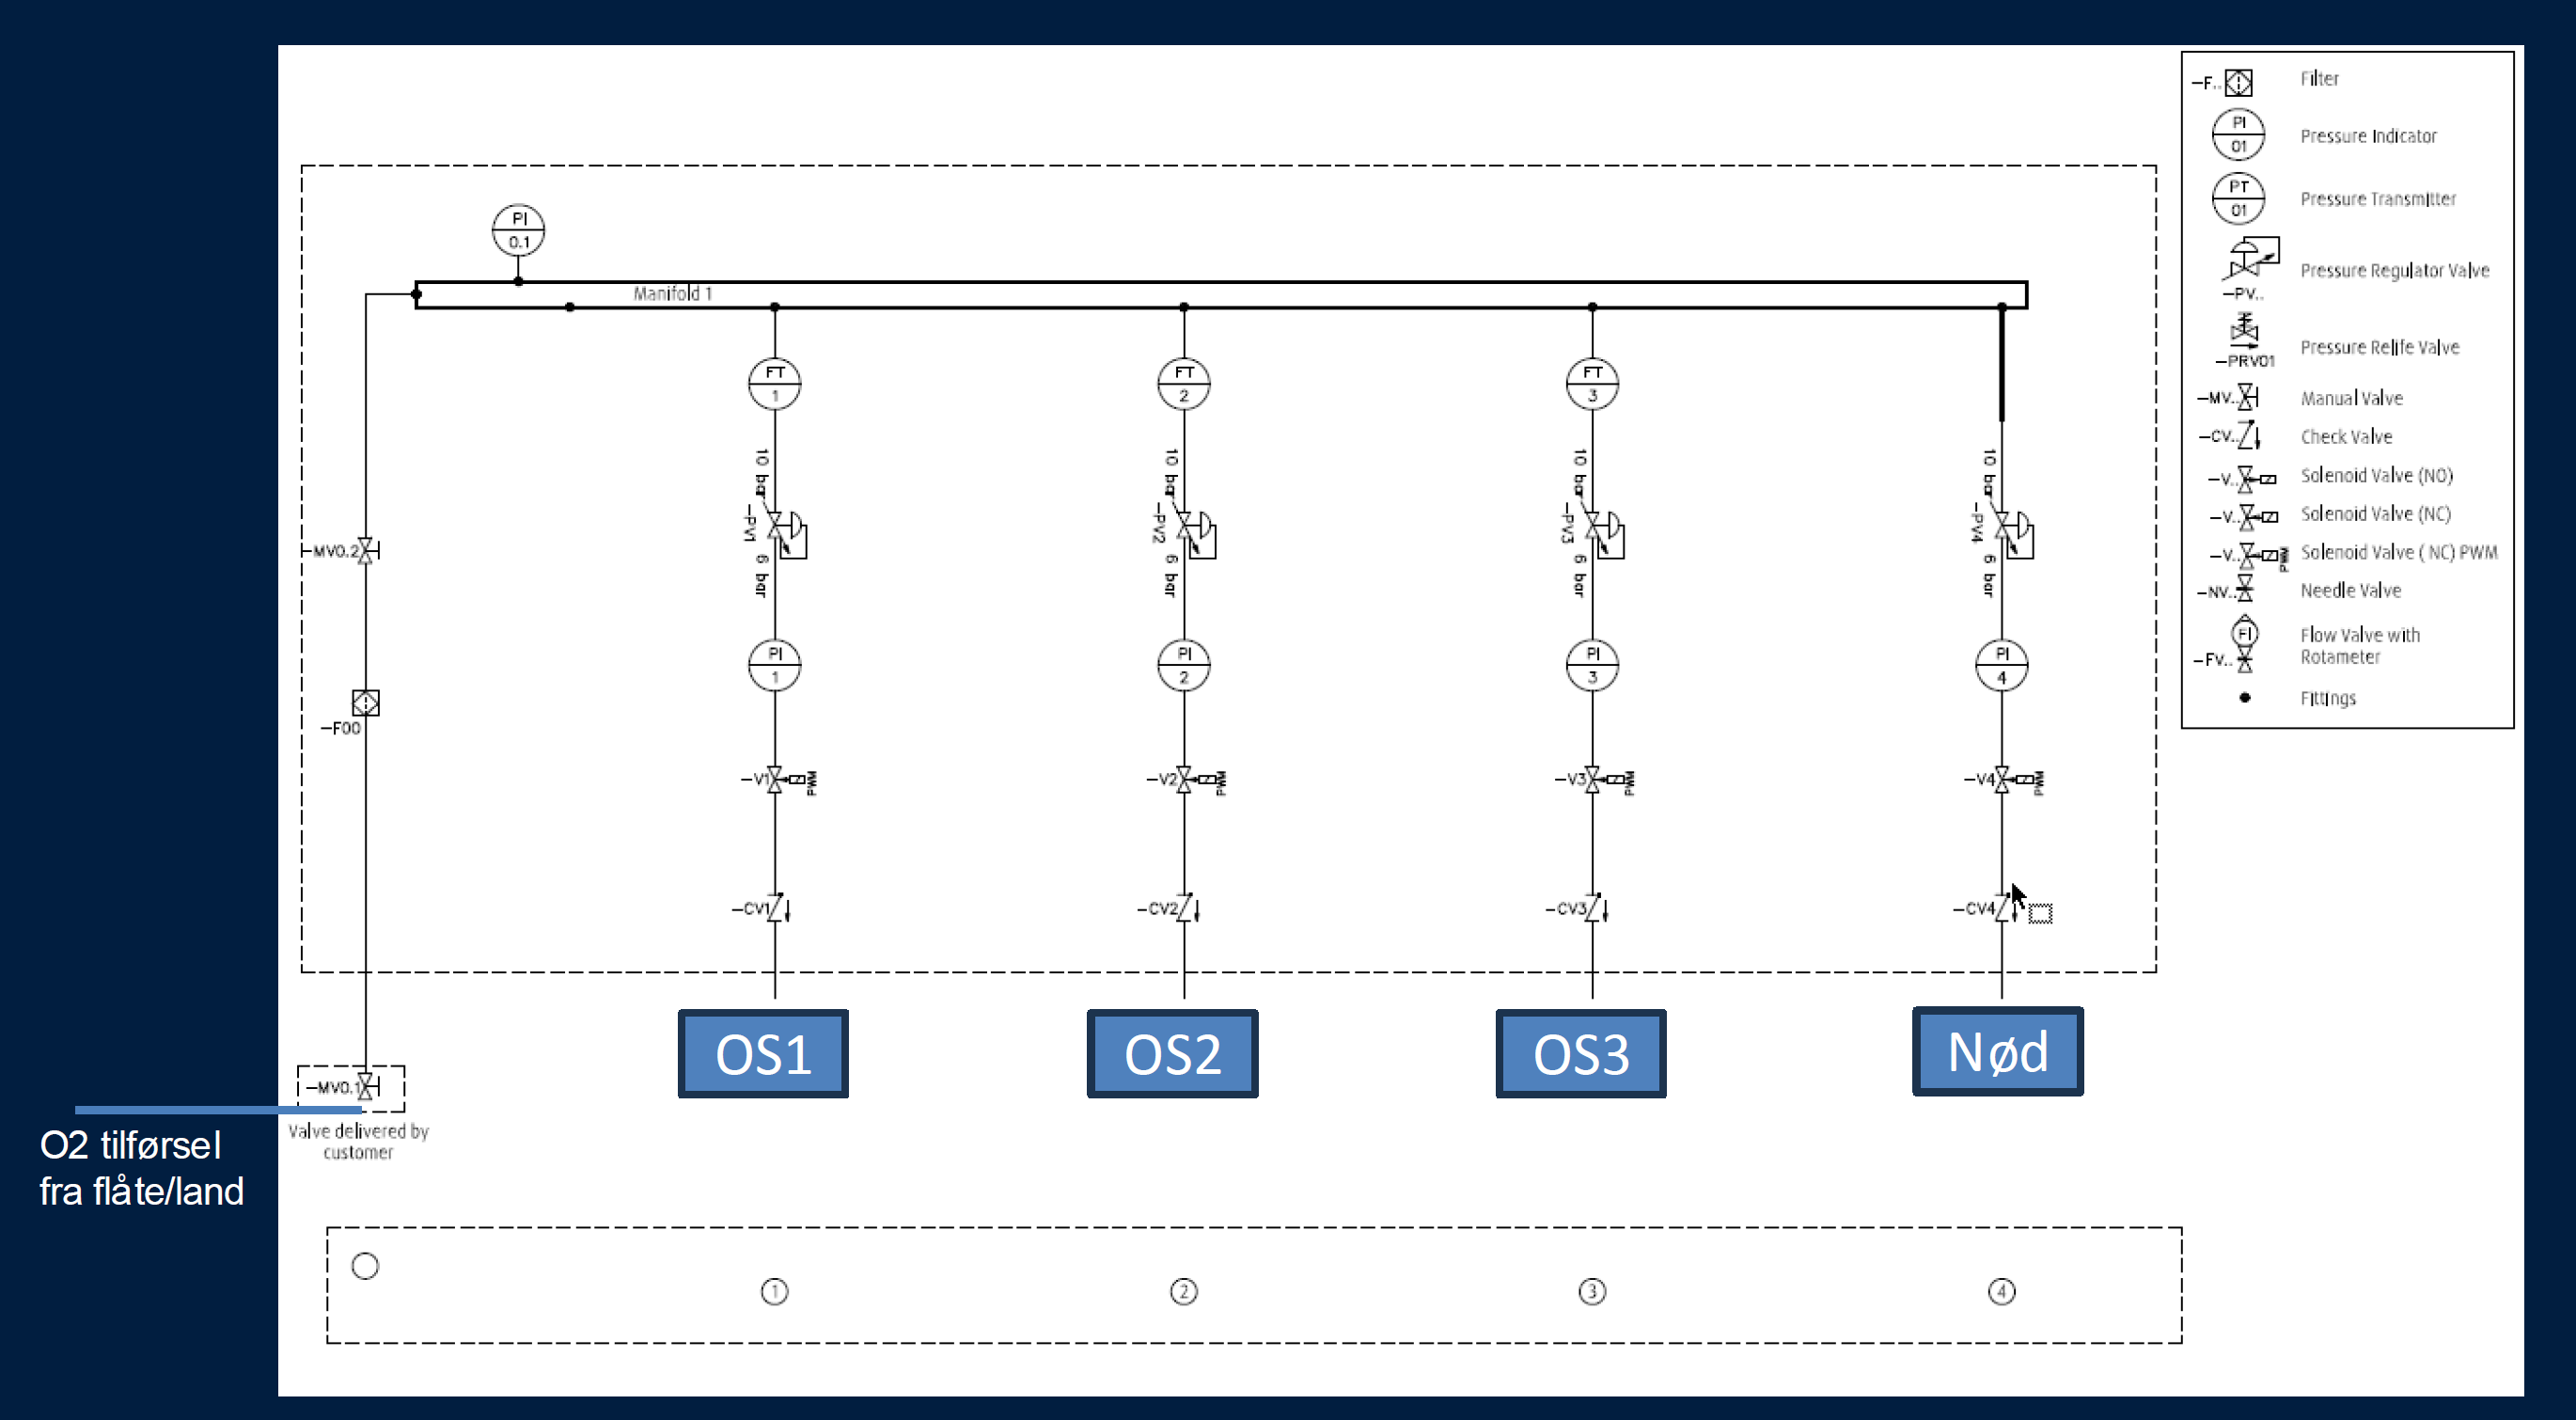
\includegraphics [width=.65\textwidth]{o2_distr_draw.png} \newline
\framebox{\parbox{\dimexpr\linewidth-2\fboxsep-2\fboxrule}{
\footnotesize \begin{enumerate}
\item<1-> Inlet pump no. 1 is running at above minimum speed.
\item<2-> We have minimum pressure at oxygen piping manifold.
\item<3-> Operator sends start signal to the oxygenator system no. 1.
\item<4-> Control valve is set to a manual predefined position.
\item<5-> Solenoid valve opens.
\item<6-> Operator sends "auto mode" signal.
\item<7-> Operator changes set point to the desired oxygen concentration.
\item<8-> Operator verifies that the valve control signal and oxygen concentration levels are stable and moving towards a stationary value.
\end{enumerate}
\textbf{Finish}
\vspace{0.1cm}
\hrule
\vspace{0.1cm}
Scenario 3 - Start oxygenator system from cold start to auto mode
  }}

\end{frame}


\end{document}